\documentclass[11pt, oneside]{article} 
\usepackage{geometry}
\geometry{letterpaper} 
\usepackage{graphicx}
	
\usepackage{amssymb}
\usepackage{amsmath}
\usepackage{parskip}
\usepackage{color}
\usepackage{hyperref}

\graphicspath{{/Users/telliott/Github-Math/figures/}}
% \begin{center} \includegraphics [scale=0.4] {gauss3.png} \end{center}

\title{Linear equations}
\date{}

\begin{document}
\maketitle
\Large

%[my-super-duper-separator]

A linear equation is a simple equation containing $x$ but no higher powers of $x$, for example, no term like $x^2$.  A very common form is to write 
\[ y = mx + b \]

The graph of this equation is a straight line, and $m$ is the \emph{slope} of the line.  When we come to quadratics $m$ will be used for something else, so here I want to use $k$ instead.  Also, $b$ is the $y$-intercept, the $y$-value when $x = 0$.  This is usually called $y_0$.  

Hence we write
\[ y = kx + y_0 \]
as the standard form.  This is called the \emph{slope-intercept} form of the equation.  

If we know one point on the line and also the slope, we can figure out the $y$-intercept.  For example, if the slope is $k=2$ and the point $(3,7)$ is on the line then
\[ 7 = 2 \cdot 3 + y_0 \]
\[ y_0 = 1 \]
so the equation of the line is
\[ y = 2x + 1 \]

Alternatively, if we know \emph{two} points on the line, $(x,y)$ and $(x',y')$, that's enough to find the slope since
\[ y = k x + y_0 \]
\[ y' = k x' +  y_0  \]
\[ y - y' = k (x - x') \]
\[ \frac{y - y'}{x - x'} = k  = \frac{\Delta y}{\Delta x} \]
And then we find $y_0$ in the same way as previously.  The slope is often called $\Delta y/\Delta x$, as indicated above.

This is called the \emph{point-slope} form of the equation.

And of course, if we know the slope $k$ and also $y_0$, then we're good.

In the figure below is the graph of the equation $y = 2x + 1$ together with a second equation $y = 0.5x + 4$.  
\begin{center} 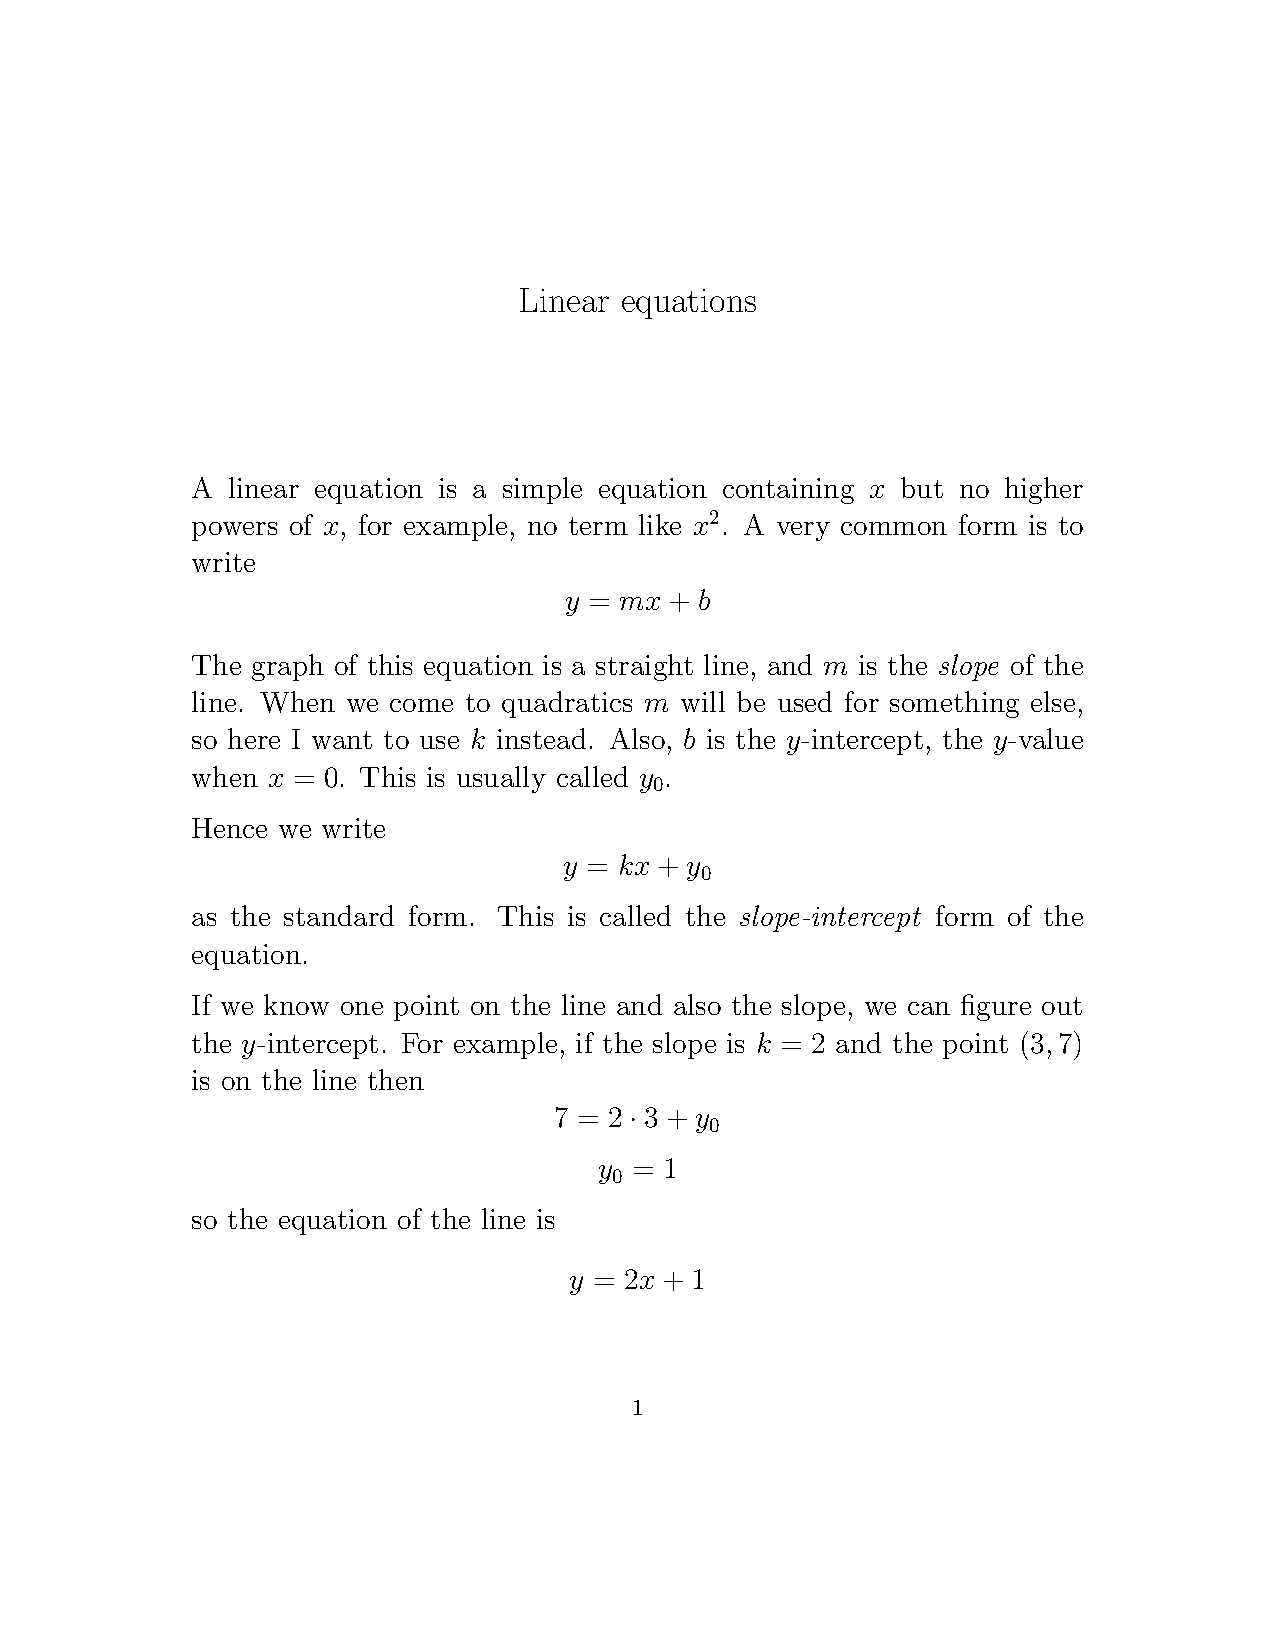
\includegraphics [scale=0.4] {linear.png} \end{center}

The point where the two lines cross is $(2,5)$.  This point solves \emph{both} equations, which is easily verified.  If $x = 2$ then we have
\[ y = 2 \cdot 2 + 1 = 5 \]
\[ y = 0.5 \cdot 2 + 4 = 1 + 4 = 5 \]

One great advantage of the graph is to see how it can happen that two linear equations have \emph{no solution}.  This occurs if the two equations are exact multiples like
\[ y = 2x + 1 \ \ \ \ \ \ 2y = 4x + 2 \]

The other way it can happen is if two equations have the same the same slope $k$, but different values for $y_0$.  This is the case where the two lines are parallel.

Suppose we have
\[ y = 2x + 1 \ \ \ \ \ \ \ y = 2x + 3 \]
We're looking to find $(x,y)$ solving both equations.  Subtract to obtain $0  = -2$.  That's definitely a problem.

Our conclusion is that when we have two unknowns $x$ and $y$, and two equations that relate them, unless they are parallel lines (or superimposed), we can find the solution.  The general principle is that if we have $n$ unknowns, we need $n$ \emph{independent} equations.

In \emph{linear algebra} we are interested in methods of solving \emph{systems of equations}.  For two equations in two unknowns, the best method is the following.  Set $y = y$ (or $x = x$, if that's more convenient), and grind through the algebra.

We're looking for a single $x$ and $y$ such that both of these are true:
\[ y = 2x + 1 \ \ \ \ \ \ y = 0.5x + 4 \]

One way is to just say $y = y$ so then
\[ 2x + 1 = 0.5x + 4 \]
\[ 1.5x = 3 \]
\[ x = 2 \]
We find $y = 5$ from the first equation, and then check that $(x,y) = (2,5)$ solves both.

Another way to do the same thing is to subtract:
\[ y = 2x + 1 \]
\[ y = 0.5x + 4 \]
Subtract the second from the first:
\[ 0 = \frac{3}{2} \ x - 3 \]
\[ \frac{3}{2} \ x = 3 \]
\[ x = 2 \]
Or you could even subtract $4$ times the second from the first:
\[ -3y = -15 \]
\[ y = 5 \]

You only need to do one of these.  Plug into one of the equations to find the other variable, and use the second equation to check your answer.

\subsection*{other special cases}
We talked about superimposed lines and parallel lines.  There are a couple other special cases.  One is a horizontal line.  Then $y$ does not depend on $x$, it's the same everywhere so
\[ y = y_0 \]
The second is a vertical line.  Then $x$ is the same everywhere, which means that $\Delta x$ is zero, so we cannot compute a slope $\Delta y / \Delta x$.
We can still write an equation, namely $x = x_0$.

And the third special case is where we have two lines that are perpendicular.  If we have
\[ y = k_1 x + r \]
\[ y = k_2 x + s \]
Then, the two lines are perpendicular when the product of the slopes is $-1$:
\[ k_1 \cdot k_2 = -1 \]

This is easy to prove.  \emph{Sketch}.  Draw a vertical line near the intersection of two perpendicular lines to form two similar right triangles.  Form the ratios of the corresponding sides and then recognize that one of those ratios is the negative of the slope of the line that points down (going left to right as usual).

\subsection*{general solution}
Let's work through the general solution for two equations using letters for the coefficients and the values of $y_0$.  We will rearrange the equations to a new form which has $x$ and $y$ on one side and $-y_0$ on the other.

Like this:
\[ ax + by = p \]
\[ cx + dy = q \]
To eliminate $y$, we need it to have the same cofactors in both equations.

To achieve this, multiply the first equation by $d$ and the second by $b$.  (I like to keep the letters in alphabetical order).
\[ adx + bdy = dp \]
\[ bcx + bdy = bq \]
Subtract
\[ (ad - bc)x  + 0 = dp - bq \]
\[ x = \frac{dp - bq}{ad - bc} \]

On the other hand, if we want to compute $x$, multiply the first equation by $c$ and the second by $a$:
\[ acx + bcy = cp \]
\[ acx + ady = aq \]

Now, I want to have the same denominator ($ad - bc$) so here I will subtract the first equation from the second one:
\[ (ad - bc)y = aq - cp \]
\[ y = \frac{aq - cp}{ad - bc} \]

Since the denominator matches, there are only three differences of products, called \emph{determinants}, which we will call
\[ D = ad - bc \]
\[ D_x = dp - bq \]
\[ D_y = aq - cp \]

and then
\[ x = \frac{D_x}{D} \ \ \ \ \ \ \ y = \frac{D_y}{D} \]

There is a method called Cramer's rule that supposedly makes it easier to remember how to do this calculation.  It is also called the method of the ratio of determinants.  It is much more useful when there are 3 equations and 3 unknowns.

You may wonder what this looks like when there is no solution.  You might guess that $D = 0$ would cause problems, and you would be right.  That's what happens when the two equations have the same slope.  We have $y = kx + r$ and $y = kx + s$ and then the matrix is
\[ kx - y = -r \]
\[ kx - y = -s \]
so $D = 0$, but we cannot divide by zero.

\subsection*{determinants}

Cramer's rule is part of the syllabus for Algebra 2.  

Once again, let's use letters for the coefficients of $x$ and $y$ and the constants.  Begin by writing an example of what's called a \emph{matrix}.  This one is 2 x 2, it has 2 rows and 2 columns, which is the simplest possible example.
\begin{verbatim}
 a  b
 c  d
\end{verbatim}
We compute the determinant of any 2 x 2 matrix as the product of one diagonal minus the product of the other.  It's important to do the first term down and to the right.
\[ D = ad - bc \]
We'll carry out this procedure three times in the following problem.

Say we have two equations in two unknowns $x$ and $y$.  Rearrange to this order
\[ ax + by = p \]
\[ cx + dy = q \]
Write the coefficients in a matrix
\begin{verbatim}
 a  b  p
 c  d  q
\end{verbatim}

Now, drop the last column
\begin{verbatim}
 a  b
 c  d
\end{verbatim}
and compute the determinant, which is exactly what we did before.
\[ D = ad - bc \]

We need two more determinants.  For the first one, take the 2 x 3 matrix and drop the $y$-column
\begin{verbatim}
 a  p
 c  q
\end{verbatim}
We drop the $y$ column to get the $y$-determinant.
\[ D_y = aq - cp \]

The last one has a twist.  Drop the $x$-column
\begin{verbatim}
 b  p
 d  q
\end{verbatim}
Compute the determinant but also \emph{multiply by minus} 1.
\[ D_x = pd - bq \]
To reduce confusion when comparing with what we did before switch the order of the letters in the term $pd = dp$, the result doesn't change:
\[ D_x = dp - bq \]

Now we can write the answer.  The $(x,y)$ that solves this is
\[ x = \frac{D_x}{D} \ \ \ \ \ \ y = \frac{D_y}{D}  \]

You can compare with what we had at the end of the previous section.  As I said, this method is overkill to actually solve 2 x 2 systems but becomes useful for 3 x 3.

\subsection*{example problem}

We have
\[ y = 2x + 1 \ \ \ \ \ \ \ y = 0.5x + 4 \]
which we rewrite as
\[ 2x - y = -1 \ \ \ \ \ \ \ 0.5x - y = -4 \]
so the matrix is
\begin{verbatim}
 2  -1 -1
1/2 -1 -4
\end{verbatim}

The first determinant is 
\[ D = (2)(-1) - (-1)(1/2) = -2 - (-1/2) = -3/2 \]
The second is
\[ D_y = (2)(-4) - (-1)(1/2) = -8 + 1/2 = -15/2 \]
\[ y = \frac{D_y}{D} = \frac{-15/2}{-3/2} = 5 \]

The last determinant is
\[ D_x = (-1)(-1) - (-1)(-4) = -3 \]
So
\[ x = \frac{D_x}{D} = \frac{-3}{-3/2} = 2 \]

\subsection*{elimination}

There is yet another approach called \emph{elimination} which is very important approach to solving real-world problems. The full name is Gauss-Jordan elimination.

We rewrite the equations as
\[ 2x - y = - 1 \ \ \ \ \ \ 0.5 x - y = -4  \]

And then write the coefficients in a matrix
\begin{verbatim}
 x   y  c
 --------
 2  -1 -1
1/2 -1 -4
\end{verbatim}
By which I mean the \emph{coefficient} of $x$, then the coefficient of $y$, then what's on the other side of the equals sign.

The ultimate goal of elimination is to get something like
\begin{verbatim}
 1  0  r
 0  1  s
\end{verbatim}
which would mean that $x = r, y = s$.  

Back to our problem.  Start with
\begin{verbatim}
 2  -1 -1
1/2 -1 -4
\end{verbatim}

We want to get a 1 in the first position for one of the rows.  I choose to multiply the second row by 2 to get a 1 in the first column:
\begin{verbatim}
 2 -1 -1
 1 -2 -8
\end{verbatim}
Switch rows so we have 1 in the first column of the first row.
\begin{verbatim}
 1 -2 -8
 2 -1 -1
\end{verbatim}
Add minus $2$ times the first row to the second to clear that row's first value:
\begin{verbatim}
 1 -2 -8
 0  3 15
\end{verbatim}
Divide the second row by $3$ to get 1 in the second column.
\begin{verbatim}
 1 -2 -8
 0  1  5
\end{verbatim}
The last step is to clear the second value from row 1, which we do by adding twice the second row to the first
\begin{verbatim}
 1  0  2
 0  1  5
\end{verbatim}
And that's our solution:  $x = 2, y = 5$.

The rules are that you can (i) do the same thing to each value in a row, (ii) switch the order of two rows or (iii) add a multiple of any row to any other row.  At each stage you want to get a 1 in the row and column that lies on a diagonal, and then clear all the values in that column.

This hardly seems worth the trouble for a simple system with only two unknowns.  But it's straightforward for say, 10 equations and 10 unknowns.  And it's easy to program computers to do this.  As we said, this subject is called \emph{linear algebra}.

\end{document}
